\documentclass{standalone}
\usepackage{tikz}
\usetikzlibrary{patterns, angles}

\begin{document}
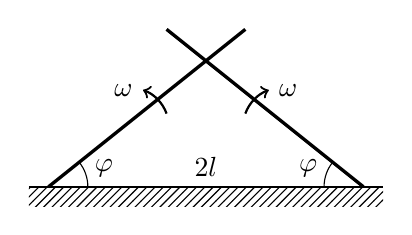
\begin{tikzpicture}
	\coordinate (A) at (0, 0);
    \coordinate (B) at (4, 0);
    \coordinate (C) at (2.5, 2);
    \coordinate (D) at (1.5, 2);
           
	\draw [draw=none, pattern=north east lines] (4.25,0) rectangle (-0.25,-0.25);
	\draw [thick] (-0.25,0) -- (4.25,0) node [midway, above] {$2l$};
	\draw (A) -- (B);
	\draw [very thick] (A) -- (C);		
	\draw [very thick] (B) -- (D);	
	\pic [draw, -, angle eccentricity=1.5] {angle = B--A--C};
	\node [right=20pt, above] at (A) {$\varphi$};
	\pic [draw, -, angle eccentricity=1.5] {angle = D--B--A};
	\node [left=20pt, above] at (B) {$\varphi$};
	\draw [thick, ->] (1.5, 0.93) arc (20:70:0.5) node [left] {$\omega$};	
	\draw [thick, ->] (2.5, 0.93) arc (160:110:0.5) node [right] {$\omega$};		
	\end{tikzpicture}
\end{document}